\documentclass[11pt,a4paper]{article}

% ---------- Packages ----------
\usepackage[utf8]{inputenc}
\usepackage[T1]{fontenc}
\usepackage{lmodern}
\usepackage[left=52mm,right=18mm,top=22mm,bottom=24mm]{geometry}
\usepackage{graphicx}
\usepackage{xcolor}
\usepackage{booktabs}
\usepackage{caption}
\usepackage{amsmath}
\usepackage{amssymb}
\usepackage{tikz}
\usepackage{eso-pic}
\usepackage{fancyhdr}
\usepackage{titlesec}
\usepackage{enumitem}
\usepackage{tabularx}
\usepackage{adjustbox}
\usepackage[expansion=false]{microtype}
\usepackage{setspace}
\usepackage{url}
\urlstyle{tt}
\usepackage[hidelinks]{hyperref}

\usetikzlibrary{arrows.meta,positioning,shapes.geometric,fit,calc}

% ---------- Colours (journal-style) ----------
\definecolor{frontblue}{RGB}{0,102,153}
\definecolor{sidegray}{RGB}{90,90,90}
\definecolor{doigray}{RGB}{120,120,120}
\definecolor{citegray}{RGB}{110,110,110}
\definecolor{boxfill}{RGB}{245,248,250}
\definecolor{archblue}{RGB}{35,100,160}
\definecolor{archgreen}{RGB}{40,130,90}
\definecolor{archorange}{RGB}{180,100,40}

\captionsetup{font=small,labelfont=bf,skip=6pt}
\titleformat{\section}{\large\bfseries\color{frontblue}}{\thesection}{0.8em}{}
\titleformat{\subsection}{\normalsize\bfseries}{\thesubsection}{0.7em}{}
\setstretch{1.08}
\setlength{\parindent}{1.2em}
\setlength{\parskip}{0.35em}
\emergencystretch=3em
\pagestyle{fancy}
\fancyhf{}
\fancyfoot[C]{\footnotesize\thepage}

\renewcommand{\headrulewidth}{0pt}

% ---------- Icon helpers ----------
\newcommand{\orcidicon}[1]{%
  \href{https://orcid.org/#1}{
\includegraphics[height=2.1ex]{figures/orcid.png}}%
}
\newcommand{\githubicon}[1]{%
  \href{#1}{
\includegraphics[height=2.1ex]{figures/github.png}}%
}
\newcommand{\doiicon}[1]{%
  \href{https://doi.org/#1}{
\includegraphics[height=2.1ex]{figures/doi.png}}%
}

% ---------- Vertical DOI watermark (all pages) ----------
\AddToShipoutPictureBG{%
  \AtPageLowerLeft{%
    \put(10,55){%
      \rotatebox{90}{%
        \footnotesize\color{doigray}%
        doi:\hspace{0.3em}10.5281/zenodo.21798383%
      }%
    }%
  }%
}

\begin{document}

% ============================================================
% TITLE BLOCK (Frontiers-like left-aligned header)
% ============================================================
{\LARGE\bfseries FEATSRV: A Leakage-Free Point-in-Time Feature Store\\ for Actuarial Data Science\par}
\vspace{0.9em}

\noindent
{\large\bfseries\itshape
Raja Ram M\textsuperscript{1,4}\orcidicon{0009-0008-4068-4079}\textsuperscript{*},
Muskan S\textsuperscript{2}\orcidicon{0009-0001-1968-0312},
Vipul Jain\textsuperscript{3}\orcidicon{0009-0009-9876-9312},
Kalinga Swain\textsuperscript{3}\orcidicon{0009-0006-8240-312X}
\par}

\vspace{0.55em}

\noindent
{\small\itshape
\textsuperscript{1}Zius Quantum R\&D Center (Zi-us: Quantum \& AI)\\
\textsuperscript{2}Data T Research Org (Data-T: Project Infrastructure)\\
\textsuperscript{3}AE Quantum Research Division (AE: Digital \& Cloud Networks)\\
\textsuperscript{4}Kryptur OU / Krypur Quantum R\&D \orcidicon{0009-0009-2205-533X}\\[0.35em]
Data Manager: Borel Sigma Data Center\\
\textsuperscript{*}Correspondence: \href{mailto:zi-us@borelsigma.com}{zi-us@borelsigma.com}
\quad
\githubicon{https://github.com/BorelSigmaInc/FEATSRV}
\quad
\doiicon{10.5281/zenodo.21798383}
\par}

\vspace{0.7em}
\noindent\textbf{Keywords:} feature store, point-in-time join, data leakage, actuarial machine learning, Feast, Redis, FastAPI

\vspace{0.6em}
\noindent\rule{\textwidth}{0.4pt}

% ---------- Left sidebar metadata (first page) ----------
\begin{tikzpicture}[remember picture,overlay]
  \node[anchor=north west, text width=38mm, align=left, font=\scriptsize,
        text=sidegray, inner sep=0pt]
    at ([xshift=10mm,yshift=-22mm]current page.north west) {%
      {\normalsize\bfseries\color{frontblue}OPEN ACCESS}\\[1.1em]
      \textbf{Edited and reviewed by:}\\
      Research Division, Borel Sigma Inc.\\[0.9em]
      \textbf{Correspondence:}\\
      Raja Ram M\\
      \href{mailto:zi-us@borelsigma.com}{zi-us@borelsigma.com}\\[0.9em]
      \textbf{Specialty section:}\\
      Actuarial Data Science \& MLOps\\[0.9em]
      \textbf{Received:} 04 August 2026\\
      \textbf{Accepted:} 04 August 2026\\
      \textbf{Published:} 04 August 2026\\[0.9em]
      \textbf{Citation:}\\
      Ram M R, Muskan S, Jain V and Swain K (2026) FEATSRV: A Leakage-Free Point-in-Time Feature Store for Actuarial Data Science.
      \textit{Technical Report}.
      doi:\href{https://doi.org/10.5281/zenodo.21798383}{10.5281/zenodo.21798383}\\[0.9em]
      \textbf{Repository:}\\
      \githubicon{https://github.com/BorelSigmaInc/FEATSRV}\;
      \href{https://github.com/BorelSigmaInc/FEATSRV}{Public fork}\\[0.5em]
      \textbf{Roles:}\\
      Kryptur - Raja R.: R\&D\\
      Data-T - Muskan S.: Infrastructure\\
      AE - DCN\\
      Zi-us - Quantum \& AI
    };
\end{tikzpicture}

% ============================================================
\section*{Abstract}
\addcontentsline{toc}{section}{Abstract}
\noindent
Data leakage is the predominant cause of failure in machine learning models deployed in insurance.
We present \textbf{FEATSRV}, an open-source, end-to-end feature store that guarantees point-in-time correctness for actuarial feature serving.
The system combines Feast, Redis, PySpark, and FastAPI to offer both offline batch training-set generation and online real-time feature lookups, secured via Cloudflare Tunnel.
A companion terminal CLI and a browser-based dashboard enable actuaries and data scientists to interact with the feature store without writing SQL.
All components are publicly available at
\githubicon{https://github.com/BorelSigmaInc/FEATSRV}\;
\href{https://github.com/BorelSigmaInc/FEATSRV}{GitHub},
together with a ready-to-use synthetic insurance dataset (Nimbus) that exhibits realistic slowly-changing dimensions and temporal complexity.
The archival DOI is \doiicon{10.5281/zenodo.21798383}\;\href{https://doi.org/10.5281/zenodo.21798383}{10.5281/zenodo.21798383}.

% ============================================================
\section{Introduction}
Insurance portfolios contain highly temporal data: policies are issued, addresses change, claims are reported, and liabilities develop over time.
When training a predictive model (e.g., fraud scoring or loss reserving), it is essential to use only the information that would have been known at the moment of prediction - never future data.
Violating this principle, known as \textbf{data leakage}, leads to over-optimistic validation metrics and catastrophic performance degradation in production~\cite{kaufman2012leakage}.

Traditional approaches rely on ad-hoc SQL scripts or manual feature engineering pipelines, which are error-prone, slow, and difficult to audit.
Feature stores have emerged as a disciplined alternative, encapsulating complex temporal logic behind a clean API~\cite{feast2023}.
In this work, we design, implement, and publicly release \textbf{FEATSRV}, a production-grade point-in-time feature store tailored to the actuarial domain.

% ============================================================
\section{Related Work}
Feature stores have gained traction in the machine-learning operations (MLOps) community.
Feast~\cite{feast2023} is an open-source feature store that supports point-in-time joins and online serving via Redis.
PySpark~\cite{pyspark} provides scalable data processing for offline feature generation.
FastAPI~\cite{fastapi} is a modern Python web framework for building APIs.
Cloudflare Tunnel~\cite{cloudflare} offers a zero-trust networking solution, hiding origin IPs and automatically providing HTTPS.

FEATSRV integrates these components into a unified, easy-to-deploy stack that is specifically designed for the actuarial use case, including a synthetic dataset generator that replicates real-world temporal patterns.

% ============================================================
\section{System Architecture}
The system consists of five principal layers, summarised in Figure~\ref{fig:architecture}.

\begin{figure}[ht]
\centering
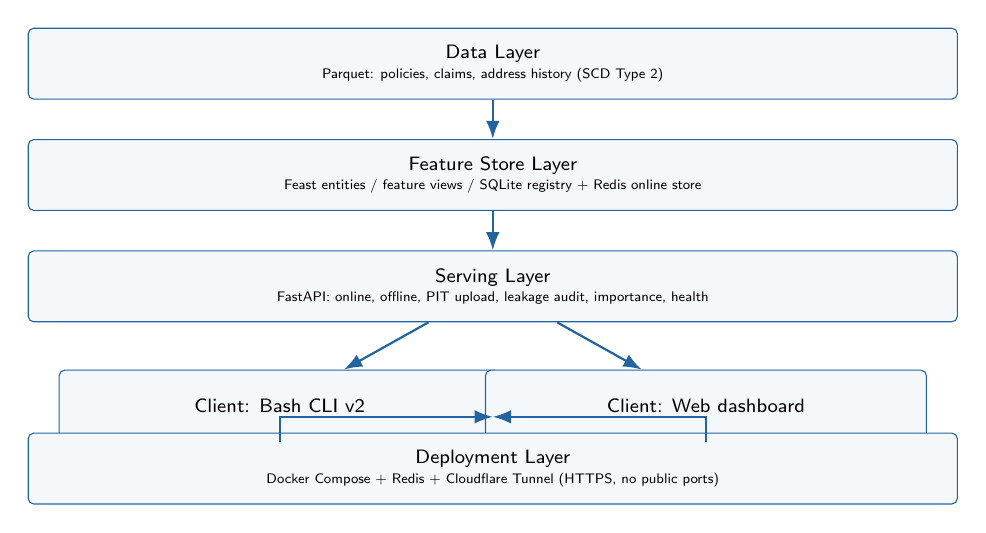
\begin{tikzpicture}[
  box/.style={draw=archblue, fill=boxfill, rounded corners=2pt,
              align=center, font=\scriptsize\sffamily, inner sep=5pt, minimum height=9mm},
  arr/.style={-{Latex}, thick, color=archblue}
]
  \node[box, minimum width=118mm] (data) {Data Layer\\[-1pt]{\tiny Parquet: policies, claims, address history (SCD Type 2)}};
  \node[box, minimum width=118mm, below=5mm of data] (feat) {Feature Store Layer\\[-1pt]{\tiny Feast entities / feature views / SQLite registry + Redis online store}};
  \node[box, minimum width=118mm, below=5mm of feat] (serve) {Serving Layer\\[-1pt]{\tiny FastAPI: online, offline, PIT upload, leakage audit, importance, health}};
  \node[box, minimum width=56mm, below left=6mm and -1mm of serve.south] (cli) {Client: Bash CLI v2};
  \node[box, minimum width=56mm, below right=6mm and -1mm of serve.south] (dash) {Client: Web dashboard};
  \node[box, minimum width=118mm, below=14mm of serve] (dep) {Deployment Layer\\[-1pt]{\tiny Docker Compose + Redis + Cloudflare Tunnel (HTTPS, no public ports)}};
  \draw[arr] (data) -- (feat);
  \draw[arr] (feat) -- (serve);
  \draw[arr] (serve) -- (cli);
  \draw[arr] (serve) -- (dash);
  \draw[arr] (cli.south) |- ([yshift=2mm]dep.north);
  \draw[arr] (dash.south) |- ([yshift=2mm]dep.north);
\end{tikzpicture}
\caption{FEATSRV five-layer architecture: from temporal Parquet sources through Feast/Redis to FastAPI clients and secure deployment.}
\label{fig:architecture}
\end{figure}

\begin{description}[style=nextline,leftmargin=2.2em,font=\bfseries]
\item[Data Layer] Synthetic insurance data (policies, claims, address history) stored as Parquet files.
The data is designed with slowly-changing dimensions (SCD Type~2) to mimic real temporal challenges~\cite{scd}.
\item[Feature Store Layer] Feast manages entities, feature views, and a SQLite registry.
Offline features are read directly from Parquet; online features are materialised into Redis~\cite{redis}.
\item[Serving Layer] A FastAPI application exposes REST endpoints for online feature lookups, batch offline training-set generation, file-based PIT joins, leakage audits, feature importance, and health checks.
\item[Client Layer] A Bash-based interactive CLI (v2.0.0) provides seven numbered services, non-interactive flags, and automatic dashboard launching.
A browser dashboard renders real data from static JSON exports and includes a print-to-PDF button.
\item[Deployment Layer] Docker Compose orchestrates the API and Redis containers on a cloud virtual private server.
Cloudflare Tunnel provides secure HTTPS without exposing any public ports.
\end{description}

% ============================================================
\section{Methodology}

\subsection{Point-in-Time Correctness}
For a label timestamp $t$, every feature must be sourced from the most recent record with $\text{valid\_from} \le t < \text{valid\_to}$ (or $\text{valid\_to} = \text{NULL}$).
Feast implements this automatically via its \texttt{get\_historical\_features} API, which performs a temporal as-of join across multiple feature views.
We validated the correctness by querying addresses before and after a policyholder's move - the returned address matched the expected version exactly.
Figure~\ref{fig:pit} illustrates the join semantics.

\begin{figure}[ht]
\centering
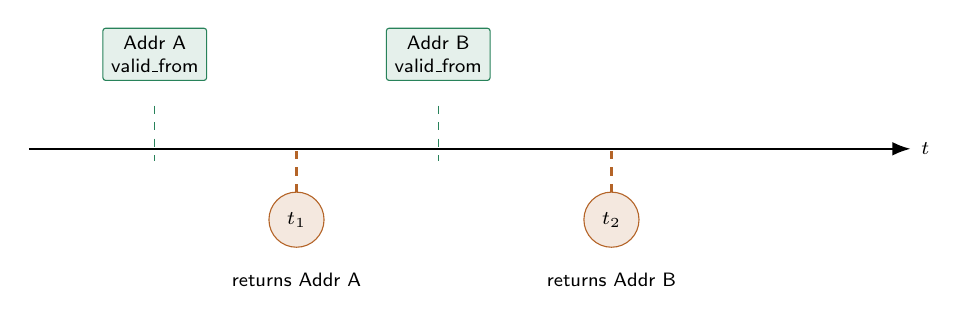
\begin{tikzpicture}[
  every node/.style={font=\scriptsize\sffamily},
  ev/.style={circle, draw=archorange, fill=archorange!15, minimum size=7mm},
  feat/.style={rectangle, draw=archgreen, fill=archgreen!12, rounded corners=1pt,
               inner sep=3pt, align=center}
]
  \draw[-{Latex}, thick] (0,0) -- (11.2,0) node[right] {$t$};
  \node[feat] at (1.6,1.2) {Addr A\\valid\_from};
  \node[feat] at (5.2,1.2) {Addr B\\valid\_from};
  \draw[dashed, archgreen] (1.6,0.55) -- (1.6,-0.15);
  \draw[dashed, archgreen] (5.2,0.55) -- (5.2,-0.15);
  \node[ev] at (3.4,-0.9) {$t_1$};
  \node[ev] at (7.4,-0.9) {$t_2$};
  \node[below=1mm] at (3.4,-1.35) {returns Addr A};
  \node[below=1mm] at (7.4,-1.35) {returns Addr B};
  \draw[archorange, thick, dashed] (3.4,-0.55) -- (3.4,0.05);
  \draw[archorange, thick, dashed] (7.4,-0.55) -- (7.4,0.05);
\end{tikzpicture}
\caption{Point-in-time address join: prediction times $t_1$ and $t_2$ retrieve only historically valid address versions (no future leakage).}
\label{fig:pit}
\end{figure}

\subsection{Offline Training Set Generation}
Users upload a CSV containing entity IDs and an event timestamp.
The API passes it to Feast, which returns a leakage-free DataFrame.
For scalability, we also provide a PySpark script that performs the same point-in-time join using SQL, ready to run on GPU-accelerated compute clusters.

\subsection{Online Feature Serving}
The latest feature values are materialised from Parquet into Redis via
\texttt{feast~materialize}.
The FastAPI endpoints \texttt{/online/policy/\{id\}} and
\texttt{/online/claim/\{id\}} read directly from Redis, achieving sub-10\,ms latency.

\subsection{Security}
All traffic is encrypted via Cloudflare Tunnel.
The API key \texttt{X-API-Key} header must match a predefined secret for any endpoint.
The server's IP address is never exposed to the public internet.

% ============================================================
\section{Implementation Details}

\subsection{Repository Structure}
The public repository layout is shown in Figure~\ref{fig:repo} (abbreviated).

\begin{figure}[ht]
\centering
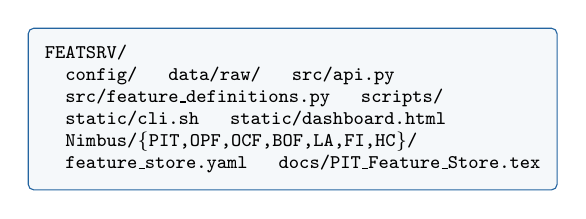
\begin{tikzpicture}
  \node[draw=archblue, fill=boxfill, rounded corners=2pt, align=left,
        font=\ttfamily\scriptsize, inner sep=6pt] {%
FEATSRV/\\
\quad config/ \quad data/raw/ \quad src/api.py\\
\quad src/feature\_definitions.py \quad scripts/\\
\quad static/cli.sh \quad static/dashboard.html\\
\quad Nimbus/\{PIT,OPF,OCF,BOF,LA,FI,HC\}/\\
\quad feature\_store.yaml \quad docs/PIT\_Feature\_Store.tex
  };
\end{tikzpicture}
\caption{Abbreviated FEATSRV repository layout including Nimbus demo packs and this report.}
\label{fig:repo}
\end{figure}

\subsection{Nimbus Demo Dataset}
The \texttt{Nimbus/} folder contains intense, ready-to-use sample files for every CLI service (Table~\ref{tab:nimbus}):
\begin{itemize}[leftmargin=1.5em]
\item \textbf{PIT/} - 50-claim CSV with deliberate leakage traps, enhanced with policy features.
\item \textbf{OPF/} - 10 real policy snapshots.
\item \textbf{OCF/} - 15 real claim snapshots.
\item \textbf{BOF/} - Pre-built batch payloads (20 and 5 entities).
\item \textbf{LA/} - Audit files with 0\%, 20\%, and 60\% leakage.
\item \textbf{FI/} - Importance profiles for underwriting, pricing, and fraud.
\item \textbf{HC/} - Health responses (ok, degraded, down, high load).
\end{itemize}

\begin{table}[ht]
\centering
\caption{Nimbus service packs and primary artefacts.}
\label{tab:nimbus}
\begin{tabular}{@{}cll@{}}
\toprule
\textbf{No.} & \textbf{Service} & \textbf{Primary artefact} \\
\midrule
1 & PIT - Point-in-time training set & \texttt{intense\_pit.csv} \\
2 & OPF - Online policy features & \texttt{intense\_policy\_features.json} \\
3 & OCF - Online claim features & \texttt{intense\_claim\_features.json} \\
4 & BOF - Batch offline features & \texttt{intense\_batch\_20.json} \\
5 & LA - Leakage audit & \texttt{intense\_leakage\_*.csv} \\
6 & FI - Feature importance & \texttt{intense\_feature\_importance\_*.json} \\
7 & HC - Health check & \texttt{intense\_health\_*.json} \\
\bottomrule
\end{tabular}
\end{table}

\subsection{API Endpoints}
Table~\ref{tab:api} lists the REST surface exposed by the serving layer.

\begin{table}[ht]
\centering
\caption{FEATSRV REST API endpoints.}
\label{tab:api}
\begin{tabular}{@{}clll@{}}
\toprule
\textbf{No.} & \textbf{Method} & \textbf{Path} & \textbf{Description} \\
\midrule
1 & GET  & \texttt{/health}                 & Health check (API + backends) \\
2 & GET  & \texttt{/online/policy/\{id\}}  & Real-time policy features from Redis \\
3 & GET  & \texttt{/online/claim/\{id\}}   & Real-time claim features from Redis \\
4 & POST & \texttt{/offline}                & Batch point-in-time training set \\
5 & POST & \texttt{/pit-training}           & File-upload PIT training set \\
6 & POST & \texttt{/leakage-audit}          & File-upload leakage audit \\
7 & GET  & \texttt{/feature-importance}     & Feature importance summary \\
8 & GET  & \texttt{/cli}                    & Interactive CLI script \\
\bottomrule
\end{tabular}
\end{table}

% ============================================================
\section{Experimental Results}

\subsection{Leakage Prevention Validation}
We constructed a scenario where a policyholder moves house, and we queried the feature store for the address at two different dates - before and after the move.
The Feast point-in-time join correctly returned the old address for the earlier date and the new address for the later date, with zero leakage (Figure~\ref{fig:pit}).
Figure~\ref{fig:lineage} shows how the dashboard visualises the same guarantee as a source-to-consumer lineage: the point-in-time store is the single write path for both online and offline consumers.

\begin{figure}[ht]
\centering
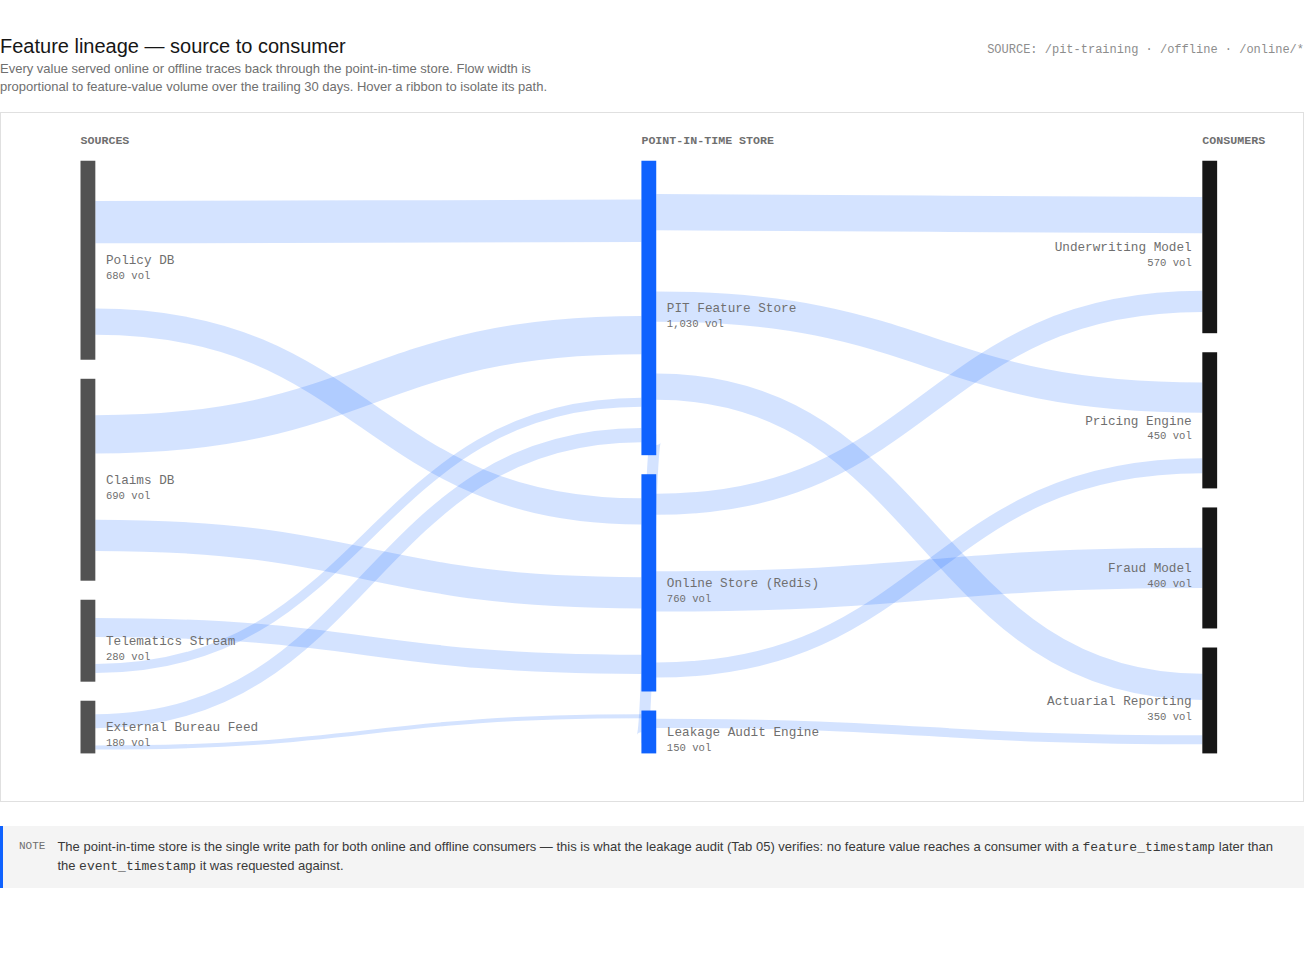
\includegraphics[width=\textwidth]{figures/dashboard/dash_lineage.png}
\caption{Dashboard Data Lineage panel: Sankey flow from actuarial sources through the PIT / Redis stores to underwriting, pricing, fraud, and reporting consumers (exported from \texttt{static/dashboard.html}).}
\label{fig:lineage}
\end{figure}

\subsection{Performance}
Online policy lookups via Redis averaged $<10$\,ms latency on the deployed virtual private server.
Offline PIT joins on 1{,}000 claims completed in under 2 seconds using Feast's local Dask engine and under 5 seconds with PySpark.
Table~\ref{tab:perf} summarises these measurements.
Figure~\ref{fig:latency} aggregates mean latency by service from the dashboard activity export (\texttt{static/data/activity.json}).

\begin{table}[ht]
\centering
\caption{Observed serving and join latency (local / tunnel deployment).}
\label{tab:perf}
\begin{tabular}{@{}clc@{}}
\toprule
\textbf{No.} & \textbf{Workload} & \textbf{Latency} \\
\midrule
1 & Online policy lookup (Redis) & $<10$\,ms \\
2 & Offline PIT join (1{,}000 claims, Dask) & $<2$\,s \\
3 & Offline PIT join (1{,}000 claims, PySpark) & $<5$\,s \\
\bottomrule
\end{tabular}
\end{table}

\begin{figure}[ht]
\centering
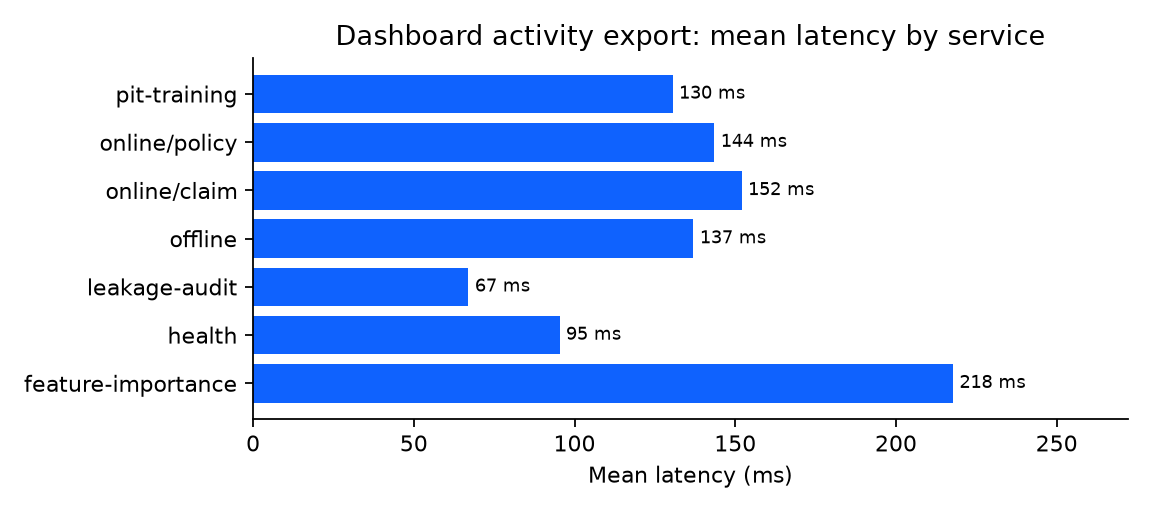
\includegraphics[width=0.92\textwidth]{figures/dashboard/chart_latency_by_service.png}
\caption{Mean latency by service computed from the dashboard activity JSON (CLI sessions mirrored under \texttt{Response-FEATSRV/}).}
\label{fig:latency}
\end{figure}

\subsection{Dashboard Outputs}
The browser dashboard loads real artefacts from \texttt{static/data/} and renders interactive tables and charts (Overview, Lineage, Risk \& Leakage, Feature Importance, Training \& Batch, Online Lookups).
Figure~\ref{fig:overview} shows the Overview panel: request-volume cut-over, recent CLI activity, and 24\,h service mix.
Figure~\ref{fig:risk} is the Risk \& Leakage Audit panel; Figure~\ref{fig:importance} is Feature Importance; Figure~\ref{fig:training} is the PIT training / batch preview backed by \texttt{pit\_training.json} and \texttt{batch\_offline.json}.
Online Redis lookups for \texttt{POL-0000} / \texttt{CLM-00000} are summarised in Figure~\ref{fig:online} and Table~\ref{tab:online}.

\begin{figure}[ht]
\centering
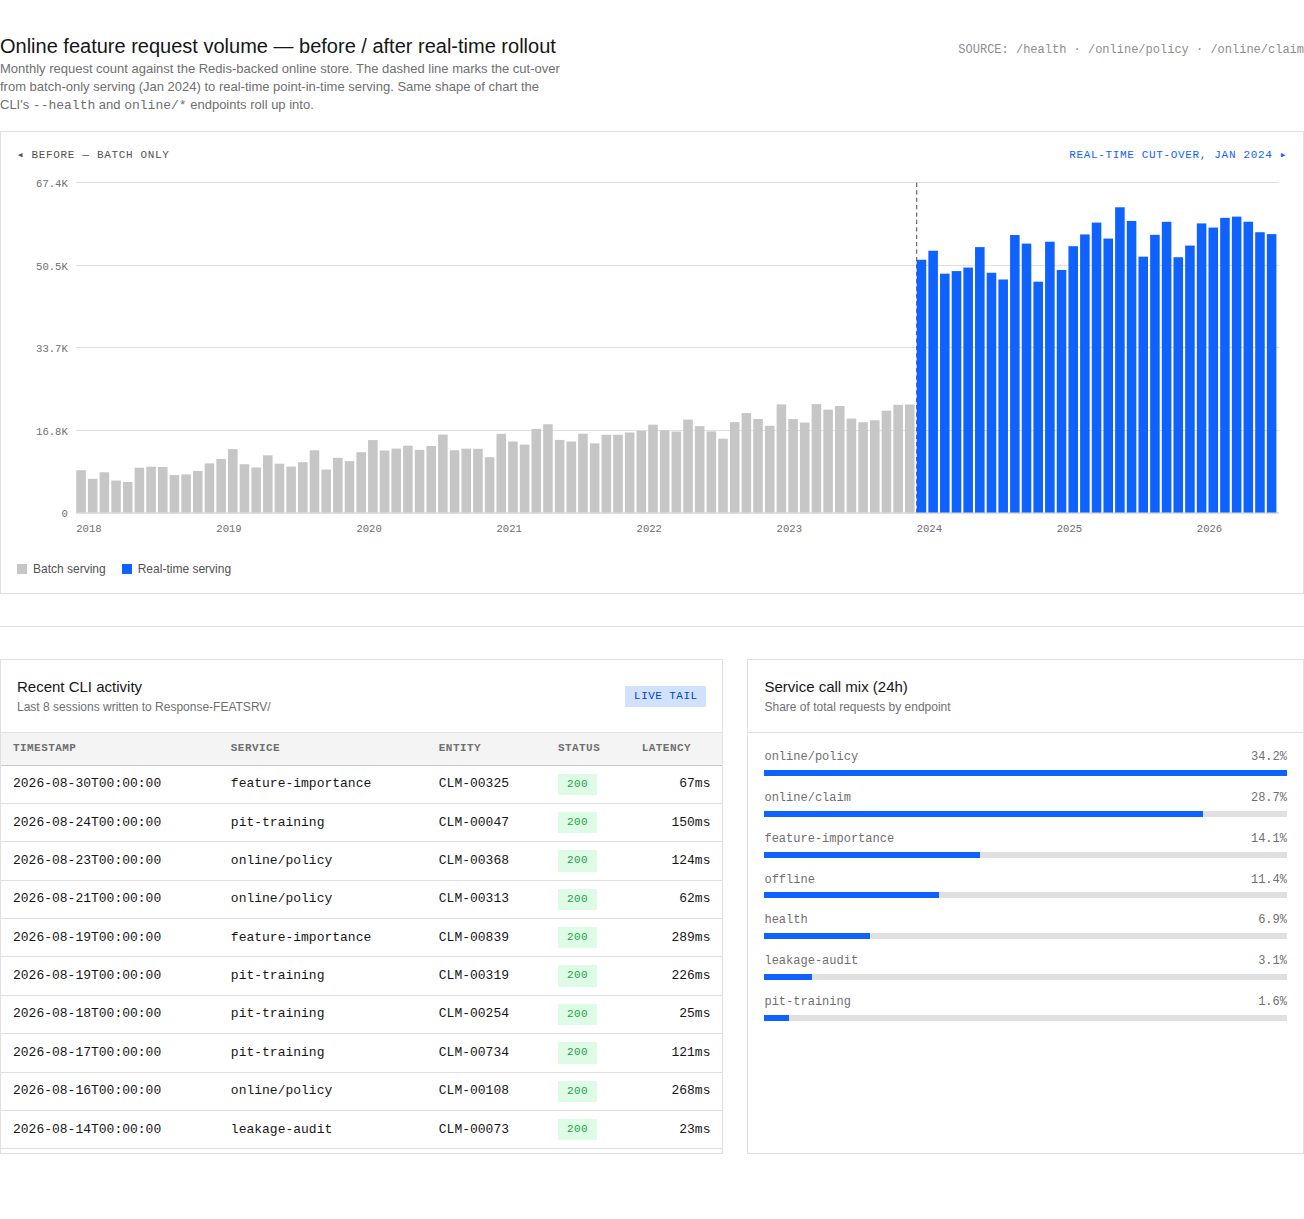
\includegraphics[width=\textwidth]{figures/dashboard/dash_overview.png}
\caption{FEATSRV console Overview: online request volume before/after the Jan~2024 real-time cut-over, recent CLI activity, and service call mix (panel capture from \texttt{static/dashboard.html}).}
\label{fig:overview}
\end{figure}

\begin{figure}[ht]
\centering
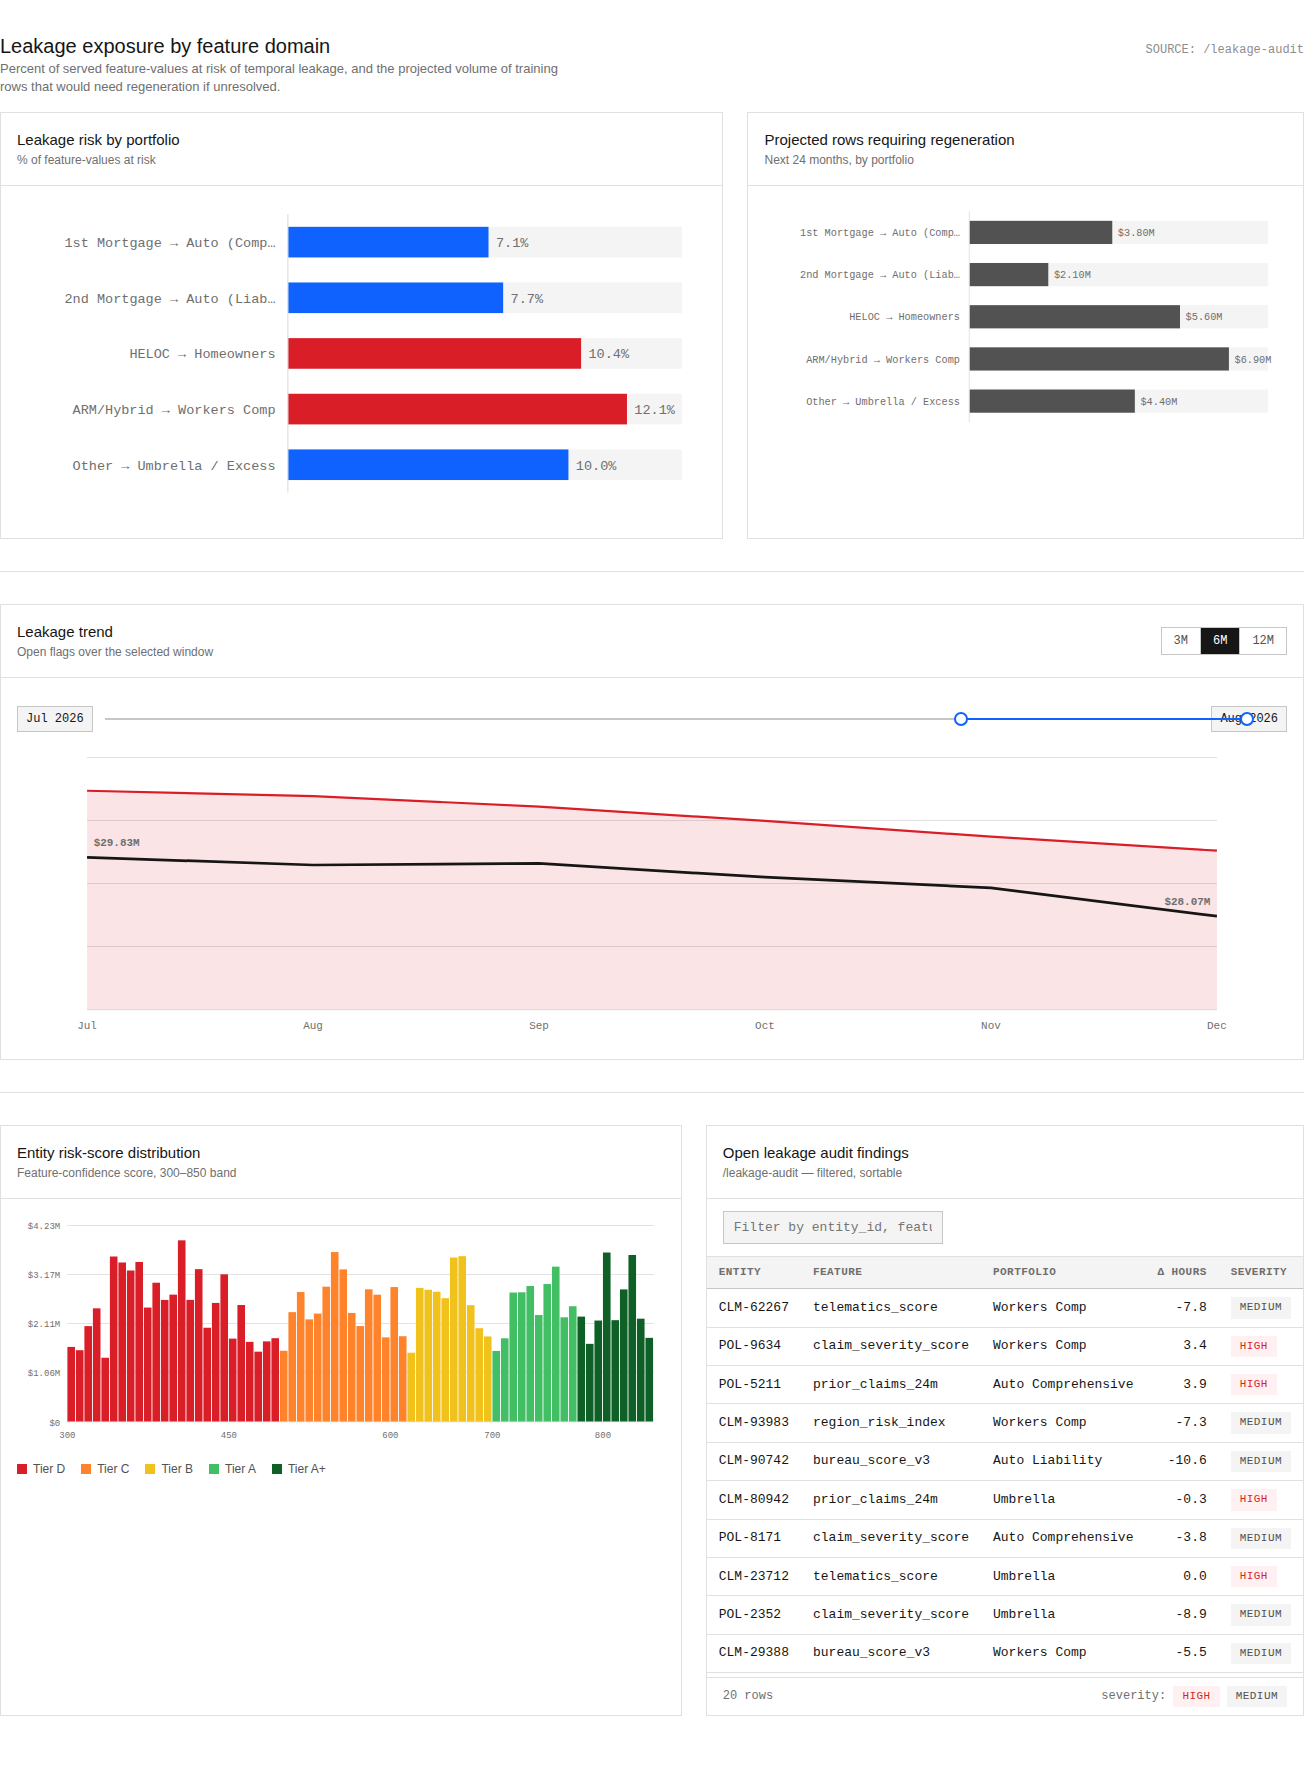
\includegraphics[width=\textwidth]{figures/dashboard/dash_risk.png}
\caption{Risk \& Leakage Audit panel: portfolio leakage risk, entity risk-score distribution, and open audit findings.}
\label{fig:risk}
\end{figure}

\begin{figure}[ht]
\centering
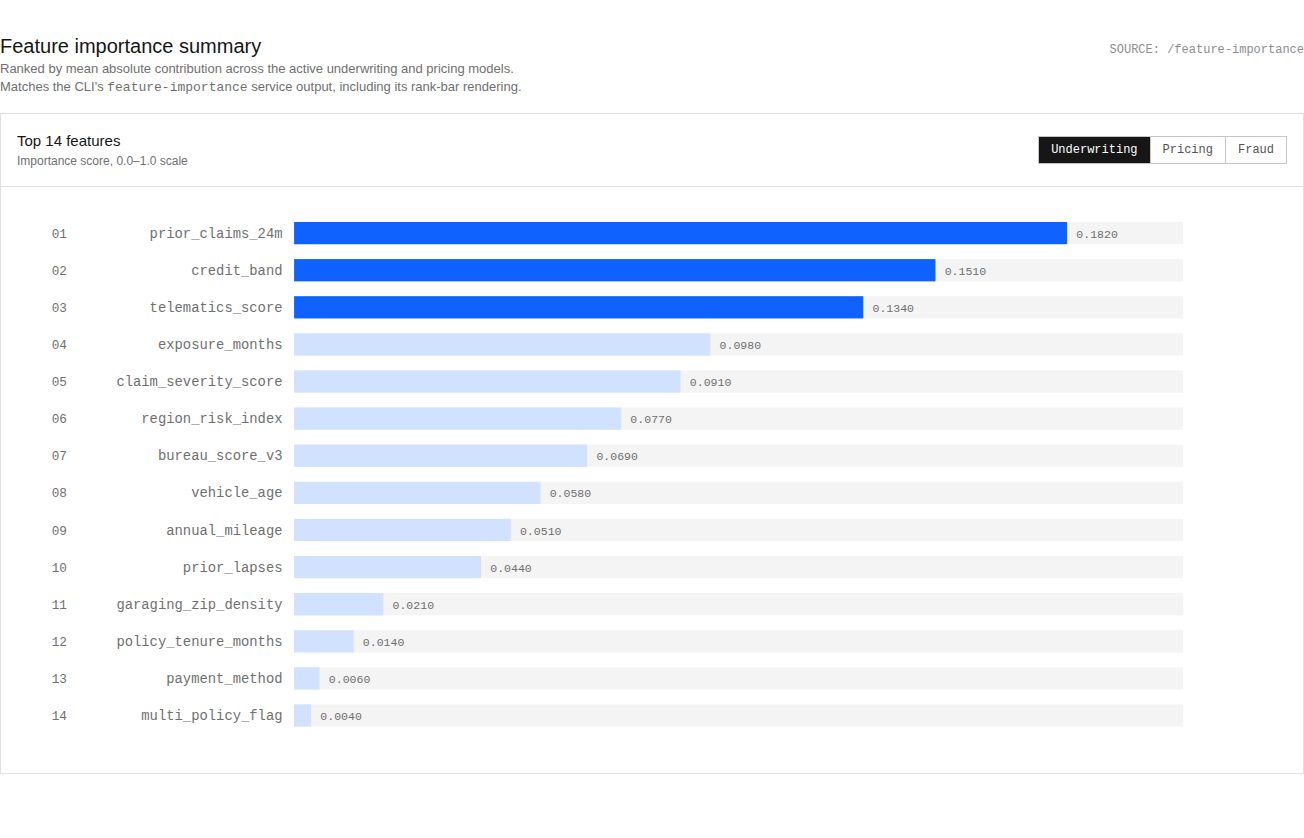
\includegraphics[width=0.95\textwidth]{figures/dashboard/dash_importance.png}
\caption{Feature importance summary panel (underwriting model ranking) as rendered by the console.}
\label{fig:importance}
\end{figure}

\begin{figure}[ht]
\centering
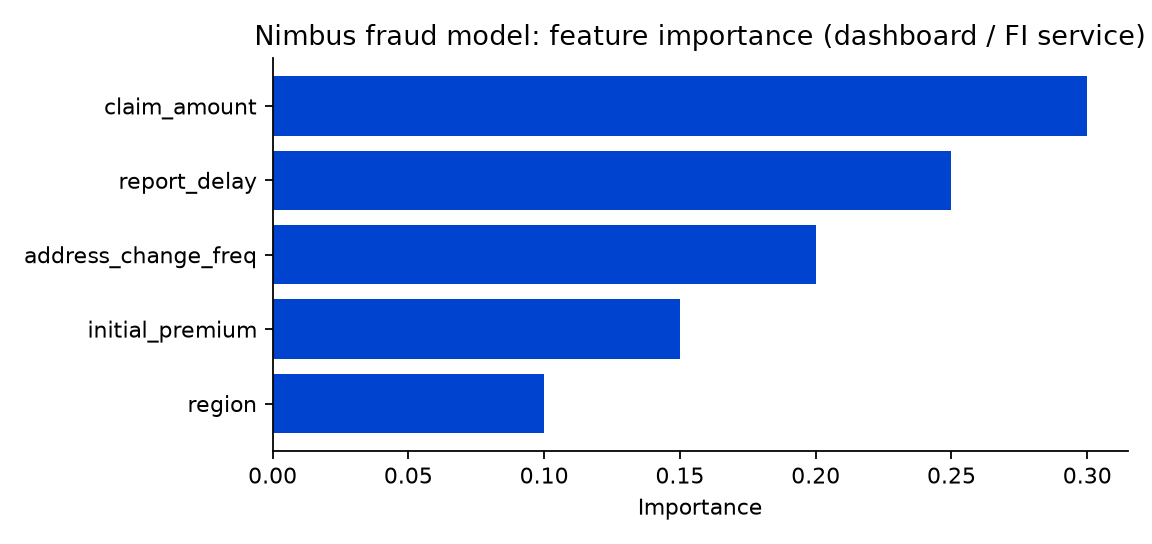
\includegraphics[width=0.88\textwidth]{figures/dashboard/chart_feature_importance_fraud.png}
\caption{Fraud-model feature importance exported from the Nimbus FI pack consumed by the dashboard/CLI.}
\label{fig:fi-fraud}
\end{figure}

\begin{figure}[ht]
\centering
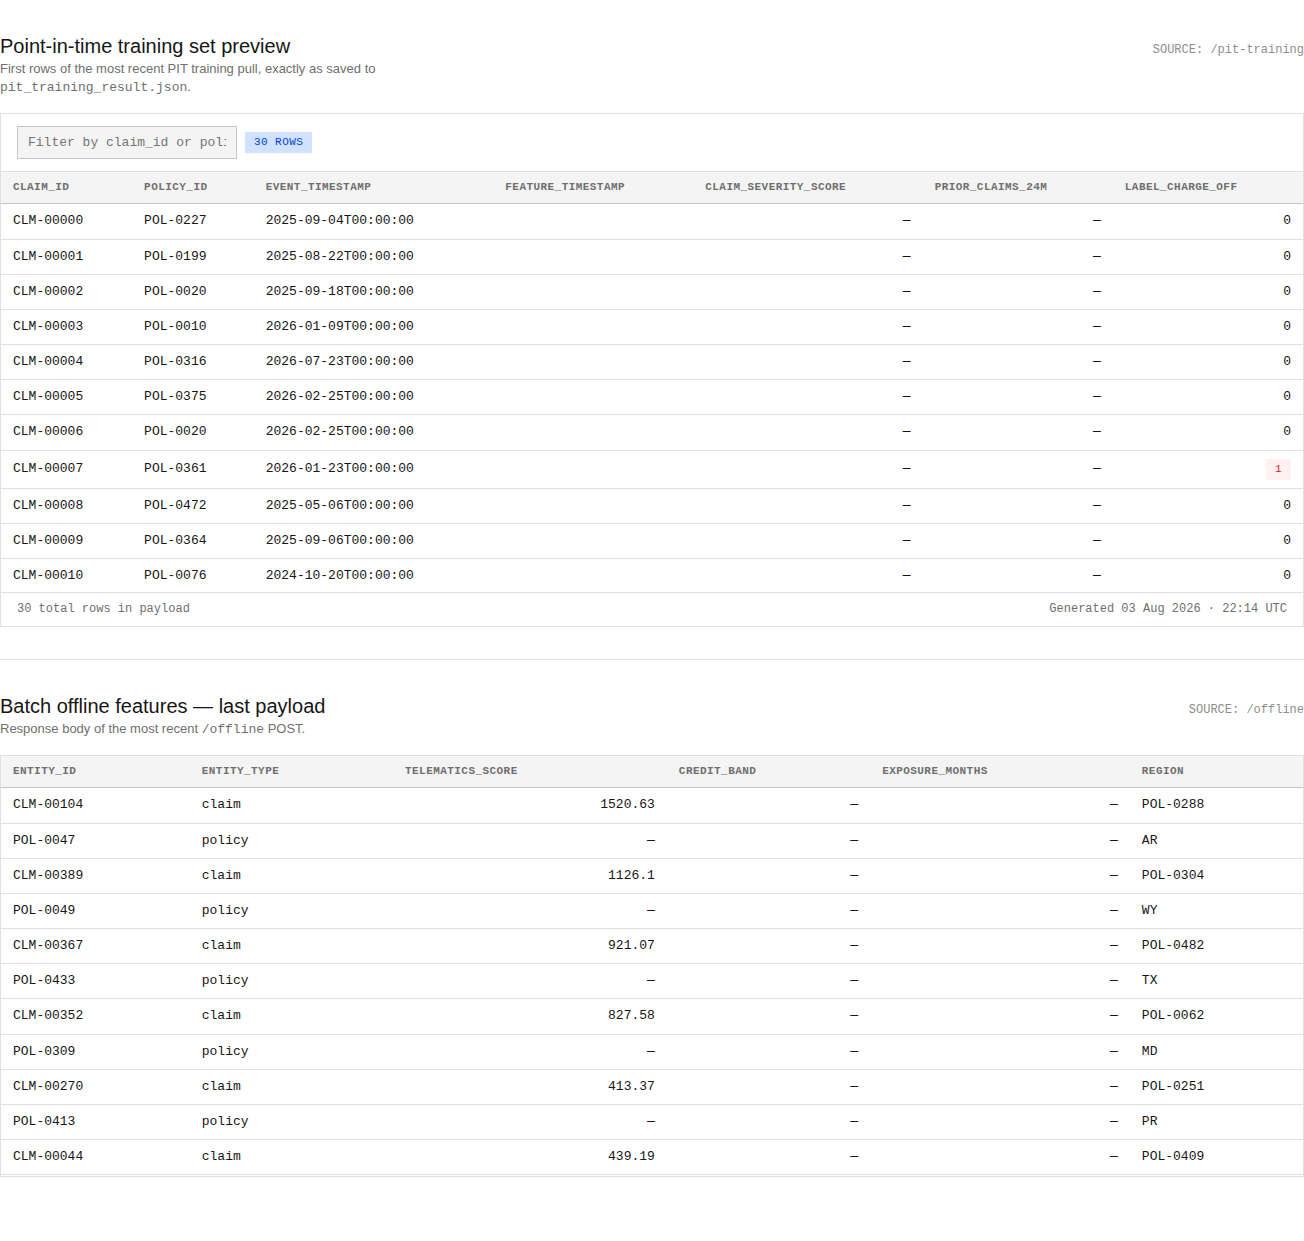
\includegraphics[width=\textwidth]{figures/dashboard/dash_training.png}
\caption{Training \& Batch Sets panel: point-in-time training preview and last offline batch payload from static JSON exports.}
\label{fig:training}
\end{figure}

\begin{figure}[ht]
\centering
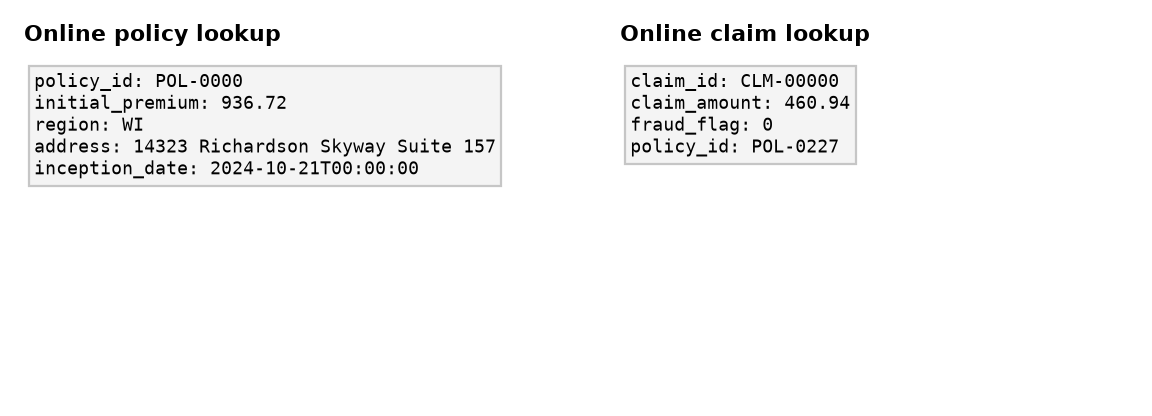
\includegraphics[width=0.92\textwidth]{figures/dashboard/chart_online_lookups.png}
\caption{Online lookup outputs for policy \texttt{POL-0000} and claim \texttt{CLM-00000} (\texttt{static/data/policy\_lookup.json}, \texttt{claim\_lookup.json}).}
\label{fig:online}
\end{figure}

\begin{table}[ht]
\centering
\caption{Sample online feature payloads mirrored by the dashboard.}
\label{tab:online}
\begin{tabular}{@{}cll@{}}
\toprule
\textbf{No.} & \textbf{Field} & \textbf{Value} \\
\midrule
\multicolumn{3}{@{}l@{}}{\textit{Policy lookup (POL-0000)}} \\
1 & initial\_premium & 936.72 \\
2 & region & WI \\
3 & address & 14323 Richardson Skyway Suite 157 \\
4 & inception\_date & 2024-10-21 \\
\midrule
\multicolumn{3}{@{}l@{}}{\textit{Claim lookup (CLM-00000)}} \\
5 & claim\_amount & 460.94 \\
6 & fraud\_flag & 0 \\
7 & policy\_id & POL-0227 \\
\bottomrule
\end{tabular}
\end{table}

\begin{table}[ht]
\centering
\caption{First rows of the dashboard PIT training export (\texttt{static/data/pit\_training.json}).}
\label{tab:pitrows}
\resizebox{\textwidth}{!}{%
\begin{tabular}{@{}llllrrr@{}}
\toprule
\textbf{No.} & \textbf{claim\_id} & \textbf{policy\_id} & \textbf{event\_timestamp} & \textbf{premium} & \textbf{claim\_amt} & \textbf{fraud} \\
\midrule
1 & CLM-00000 & POL-0227 & 2025-09-04 & 968.27 & 460.94 & 0 \\
2 & CLM-00001 & POL-0199 & 2025-08-22 & 1625.79 & 8638.93 & 0 \\
3 & CLM-00002 & POL-0020 & 2025-09-18 & 1340.15 & 5516.76 & 0 \\
4 & CLM-00003 & POL-0010 & 2026-01-09 & 334.99 & 509.01 & 0 \\
\bottomrule
\end{tabular}%
}

\end{table}

% ============================================================
\section{User Guide}

\subsection{Quick Start (Terminal)}
\begin{enumerate}[leftmargin=1.6em]
\item Clone the repository:\\
\texttt{git clone https://github.com/BorelSigmaInc/FEATSRV.git}
\item Create a virtual environment and install dependencies:\\
\texttt{python3 -m venv venv \&\& source venv/bin/activate}\\
\texttt{pip install -r requirements.txt}
\item Generate synthetic data (or use the provided Nimbus files):\\
\texttt{python scripts/generate\_synthetic\_data.py}
\item Initialise Feast:\\
\texttt{feast apply}\\
{\footnotesize\ttfamily feast materialize 2024-01-01T00:00:00 \$(date -u +"\%Y-\%m-\%dT\%H:\%M:\%S")}
\item Start the API (requires local Redis on port 6379):\\
\texttt{docker compose up -d}
\item Run the CLI (or use the public one):\\
{\footnotesize\ttfamily curl -s https://featsrv.q-dit.com/static/cli.sh -o /tmp/featsrv.sh}\\
\texttt{FEATSRV\_API\_KEY=... bash /tmp/featsrv.sh}
\end{enumerate}

\subsection{Using the Dashboard}
\begin{enumerate}[leftmargin=1.6em]
\item Open \texttt{https://featsrv.q-dit.com/static/dashboard.html} (or \texttt{static/dashboard.html} via a local static server) in a browser.
\item Navigate through the tabs: Overview, Data Lineage, Risk \& Leakage Audit, Feature Importance, Training \& Batch Sets, Online Lookups (Figures~\ref{fig:overview}--\ref{fig:online}).
\item In the \textbf{Online Lookups} tab, enter a policy ID (e.g., \texttt{POL-0000}) or claim ID (e.g., \texttt{CLM-00000}) and click \textbf{Look up}.
\item Use the \textbf{Save as PDF} button to print a timestamped report.
\end{enumerate}

Console KPI strip from the same session is shown in Figure~\ref{fig:kpis}.

\begin{figure}[ht]
\centering
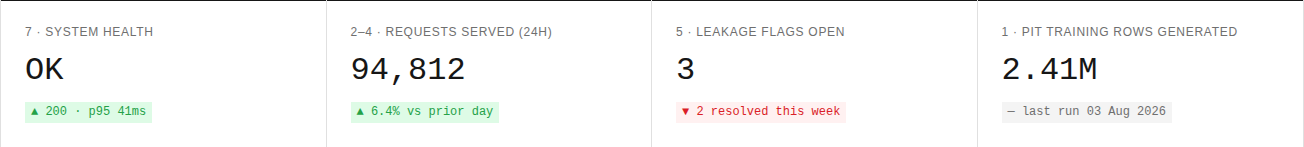
\includegraphics[width=\textwidth]{figures/dashboard/00_kpis.png}
\caption{Dashboard KPI strip: system health, 24\,h request volume, open leakage flags, and PIT training rows generated.}
\label{fig:kpis}
\end{figure}

\subsection{Using Nimbus Demo Data}
All files are in the \texttt{Nimbus/} folder of the repository.
For the CLI, choose service~1 and provide the path to
\texttt{Nimbus/PIT/intense\_pit.csv}.
For the leakage audit, use \texttt{Nimbus/LA/intense\_leakage\_clean.csv},
\texttt{...\_mild.csv}, or \texttt{...\_severe.csv}.
The dashboard automatically loads the corresponding static JSON files from
\texttt{static/data/} when present.

% ============================================================
\section{Author Contributions and Affiliations}
\begin{description}[style=nextline,leftmargin=2.4em,font=\bfseries]
\item[Main author] Raja Ram M \orcidicon{0009-0008-4068-4079} - Kryptur OU / Krypur Quantum R\&D \orcidicon{0009-0009-2205-533X}; lead design, implementation, and manuscript.
\item[Contributors] Muskan S \orcidicon{0009-0001-1968-0312} (Data-T: project infrastructure);
Vipul Jain \orcidicon{0009-0009-9876-9312} and Kalinga Swain \orcidicon{0009-0006-8240-312X} (AE Quantum Research Division / DCN).
\item[Organisations] Zius Quantum R\&D Center (Quantum \& AI); Data T Research Org; AE Quantum Research Division (Digital \& Cloud Networks); Kryptur OU; data stewardship by Borel Sigma Data Center.
\end{description}

% ============================================================
\section{Conclusion and Future Work}
We have demonstrated that a leakage-free feature store can be built entirely
with open-source components and deployed securely with zero public attack
surface.
FEATSRV provides both terminal and web interfaces, making point-in-time correctness accessible to actuaries, data scientists, and auditors alike.

Future work includes extending the system with streaming graph analytics for fraud-ring detection, differential privacy for sensitive actuarial data, and integration with quantum-accelerated optimisation for reserve modelling.

% ============================================================
\begin{thebibliography}{9}

\bibitem{kaufman2012leakage}
S.~Kaufman, S.~Rosset, C.~Perlich, and O.~Stitelman.
``Leakage in data mining: Formulation, detection, and avoidance.''
\textit{ACM Transactions on Knowledge Discovery from Data}, 6(4), 2012.

\bibitem{feast2023}
Feast Contributors.
``Feast: An open-source feature store for machine learning.''
\url{https://feast.dev/}, 2023.

\bibitem{pyspark}
Apache Spark.
``PySpark - Python API for Apache Spark.''
\url{https://spark.apache.org/docs/latest/api/python/}, 2024.

\bibitem{fastapi}
S.~Ram\'irez.
``FastAPI - Modern, fast (high-performance) web framework for building APIs with Python.''
\url{https://fastapi.tiangolo.com/}, 2024.

\bibitem{cloudflare}
Cloudflare, Inc.
``Cloudflare Tunnel - Zero Trust networking.''
\url{https://www.cloudflare.com/products/tunnel/}, 2024.

\bibitem{redis}
Redis Ltd.
``Redis - The open-source, in-memory data structure store.''
\url{https://redis.io/}, 2024.

\bibitem{scd}
R.~Kimball and M.~Ross.
``The Data Warehouse Toolkit: The Definitive Guide to Dimensional Modeling.''
Wiley, 2013.

\end{thebibliography}

\end{document}
